\chapter{Il web ad oggi}
\section{Perché ottimizzare la propria interfaccia web?}
Le tecnologie per la produzione di applicazioni web si sono evolute esponenzialmente da quando il web era ancora un progetto pensato per scambiare documentazione scientifica in modalità elettronica. Oggi il web viene utilizzato per gli scopi più disparati, dal promuovere il proprio business a offrire veri e propri servizi ad alto traffico e scalabilità.
Molte compagnie basano il proprio business esclusivamente sul mondo web, si pensi ad un sito ecommerce o a piattaforme di condivisione come i social, Chi invece gestisce business esterni sfrutta il web e le piattaforme sviluppate su di esso per promuovere la propria attività, in un contesto diventato ormai essenziale per ogni tipo di business.
\newline
Pensiamoci, qual'è  la prima cosa che facciamo quando necessitiamo di informazioni su un particolare prodotto o servizio? oppure abbiamo bisogno di riempire un vuoto informativo in maniera tempestiva?  interroghiamo l'oracolo del nuovo millennio Google in cerca di risposte.
\newline
Il mondo web si è espanso cosi tanto da diventare un qualcosa di normale e scontato nella nostra vita quotidiana e con tante realtà che ormai spostano le loro vetrine e i loro contenuti informativi su questa tecnologia, e offrono user experience sempre più avanzate, gli utenti sono diventati sempre più esigenti in termini di performance e tempi di risposta da parte di questi servizi.Secondo uno studio condotto nel 2018 da Google, la probabilita che un utente abbandoni il sito aumenta in maniera esponenziale in base al tempo di caricamento delle pagine.\cite{mobile-page-speed}
\newline
\begin{figure}[H]
\centering
   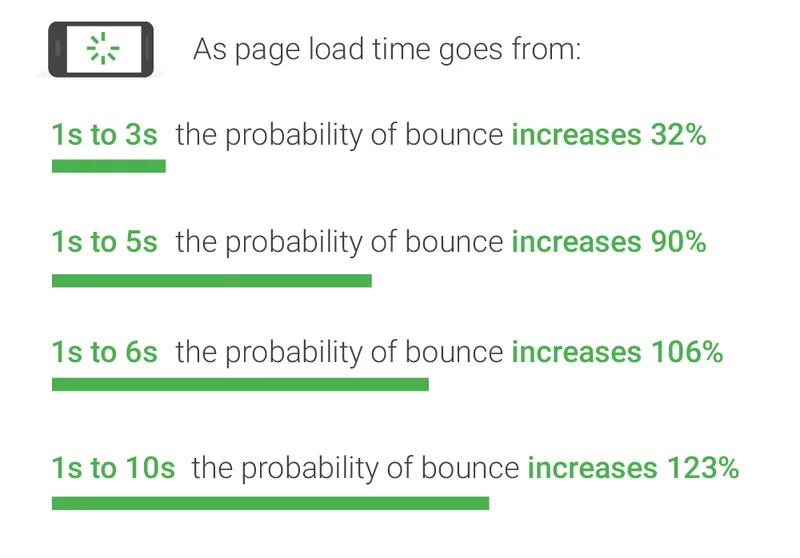
\includegraphics[scale=0.5]{resources/mobile-page-speed-new-industry.png}
\cite{mobile-page-speed}
\caption{probabilità di abbandono del sito in relazione al tempo di caricamento}
\end{figure}
Inoltre, più della metà delle richieste effettuate a questi servizi avviene da device mobile e per il 70\% dei siti analizzati i tempi di caricamento ammontano a più di 5 secondi. \cite{mobile-page-speed}

